\section{Results}
\label{sec:results}

We organise the discussion around six themes
(Sections~\ref{ssec:results-volatility}--\ref{ssec:results-robustness}).
The strongest single finding (Section~\ref{ssec:results-volatility})
is a robust and substantial increase in intraday magnitude and range
around news events, present across all assets and windows. The
directional content of LLM sentiment (Section~\ref{ssec:results-direction})
is modest, statistically detectable on a small number of windows
after FDR adjustment, and economically below transaction costs. The
remaining subsections (\ref{ssec:results-heterogeneity}--\ref{ssec:results-market-structure})
cover heterogeneity, timing, and market-structure questions, while
Section~\ref{ssec:results-robustness} reports the robustness
defences. Throughout, we report Benjamini-Hochberg $q$-values in the
text; raw $p$-values appear in the tables.

\subsection{Volatility and magnitude: events move markets}
\label{ssec:results-volatility}

We first ask whether news events are associated with abnormal
intraday movement, irrespective of direction. The answer is
unambiguously yes.

\paragraph{H1 (event vs matched baseline absolute return).}
Across both assets and all five window lengths, the mean absolute
event return exceeds the mean absolute matched-baseline return by a
factor between $1.33\times$ and $1.87\times$. The smallest ratio
occurs on the longest NDX window (240 minutes), the largest on the
shortest EUR/USD window (1 minute). All ten cells reach $q < 10^{-14}$
on a one-sided Mann-Whitney $U$ test and remain significant under a
Welch $t$-test robustness check (Online Appendix). On the primary
$5/15/60$-minute windows the event/baseline ratios are
$\{1.76, 1.69, 1.58\}$ for EUR/USD and $\{1.56, 1.57, 1.43\}$ for
NDX. See Table~\ref{tab:h1-main} and
Figure~\ref{fig:event-time-profile}, which plots the average
absolute log-return as a function of minutes from the event
timestamp; both assets show a sharp lift in the post-event window
that persists for at least four hours, with the EUR/USD ratio
larger at short horizons and the NDX ratio larger at longer
horizons.

\begin{table}[!htbp]
\centering
\caption{Event-window magnitude versus matched baseline (H1 and C2).}
\label{tab:h1-main}
\begin{threeparttable}
\small
\begin{tabular}{lcccccc}
\toprule
 & \multicolumn{3}{c}{EUR/USD (USD proxy)} & \multicolumn{3}{c}{Nasdaq-100} \\
\cmidrule(lr){2-4} \cmidrule(lr){5-7}
Window & 5m & 15m & 60m & 5m & 15m & 60m \\
\midrule
Mean $|r|$, event ($\%$) & 0.0324 & 0.0532 & 0.0993 & 0.0839 & 0.1441 & 0.2682 \\
Mean $|r|$, baseline ($\%$) & 0.0184 & 0.0314 & 0.0630 & 0.0539 & 0.0920 & 0.1874 \\
Ratio (event/baseline) & 1.76$\times$ & 1.69$\times$ & 1.58$\times$ & 1.56$\times$ & 1.57$\times$ & 1.43$\times$ \\
$q$-value (MWU one-sided) & ${<}10^{-15}$ & ${<}10^{-15}$ & ${<}10^{-15}$ & ${<}10^{-15}$ & ${<}10^{-15}$ & ${<}10^{-15}$ \\
\addlinespace
\multicolumn{7}{l}{\textit{C2: intra-window range and maximum absolute move}} \\
Range, event ($\%$) & 0.0621 & 0.1047 & 0.1995 & 0.1715 & 0.2921 & 0.5704 \\
Range, baseline ($\%$) & 0.0352 & 0.0625 & 0.1263 & 0.1054 & 0.1843 & 0.3772 \\
Ratio range & 1.76$\times$ & 1.68$\times$ & 1.58$\times$ & 1.63$\times$ & 1.59$\times$ & 1.51$\times$ \\
Max abs move, event ($\%$) & 0.0499 & 0.0839 & 0.1577 & 0.1353 & 0.2308 & 0.4491 \\
Ratio max abs move & 1.76$\times$ & 1.68$\times$ & 1.57$\times$ & 1.62$\times$ & 1.58$\times$ & 1.53$\times$ \\
\addlinespace
$N$ clusters (event) & 1,288 & 1,273 & 1,208 & 1,200 & 1,178 & 1,099 \\
\bottomrule
\end{tabular}
\begin{tablenotes}
\footnotesize
\item \textit{Notes.} Event-window absolute return $|r|$, intra-window
high-low range, and maximum absolute intra-window move, all in percentage
points. Baselines are drawn from non-event windows matched on asset,
window length, hour-of-day, and day-of-week, with 30 draws per event.
The $q$-value comes from a one-sided Mann-Whitney $U$ test against
the baseline distribution, with Benjamini-Hochberg FDR adjustment
applied across the full hypothesis battery. Cluster identifier groups
events at a 15-minute gap. Welch $t$-test alternative reported in
the Online Appendix.
\end{tablenotes}
\end{threeparttable}
\end{table}


\begin{figure}[!htbp]
\centering
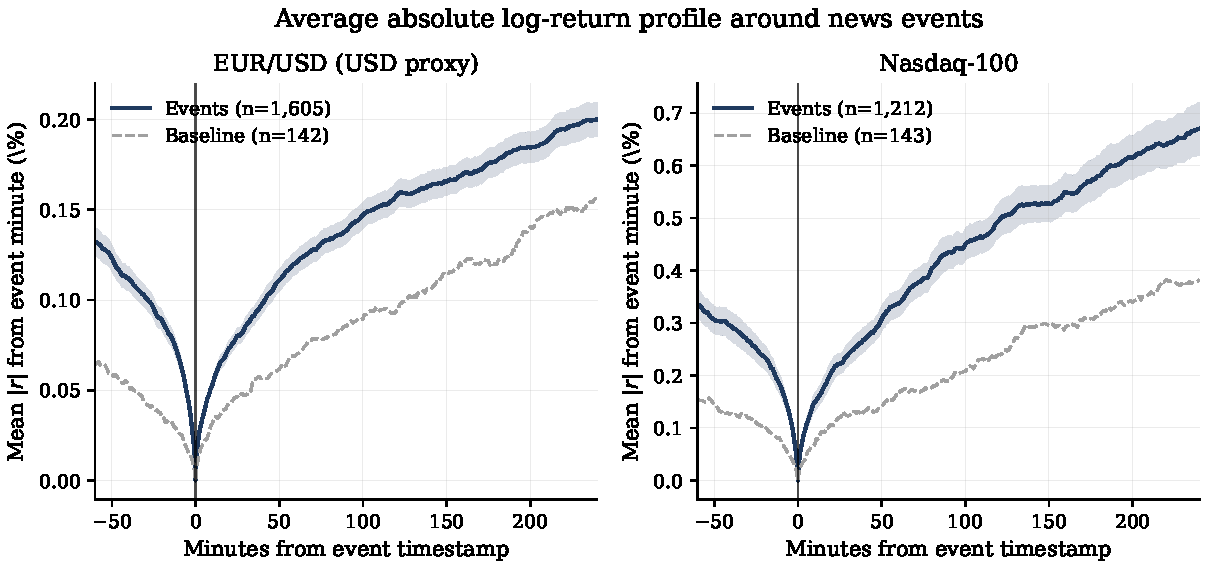
\includegraphics[width=\textwidth]{figures/figure_1_event_time_profile.pdf}
\caption{Average $|r|$ around news events, with $r$ defined as the
log price change from the event minute. Solid line: $2{,}449$
events; dashed line: baseline of random non-event windows of the
same length. Shaded area: $\pm 1.96$ standard errors around the
event mean. The vertical line marks the event timestamp.}
\label{fig:event-time-profile}
\end{figure}

\paragraph{C2 (range and maximum absolute intra-window move).}
The intra-window range and the maximum absolute move are even more
strongly elevated than the close-to-close return. For EUR/USD the
range/baseline ratio is $1.76\times$ at 5 minutes and $1.58\times$
at 60 minutes; for NDX the corresponding values are $1.63\times$ and
$1.51\times$. All twenty cells in this table reach $q < 10^{-30}$.
The economic interpretation is that news events generate
intra-window excursions that close-to-close returns understate,
often because the price overshoots and partially reverses within
the same window. This is the single most useful new result of the
analysis and we recommend that practitioners reading the paper
attend to it more than to any of the direction-based tests.
Figure~\ref{fig:range-ratios} plots the three magnitude ratios
side by side; both range and maximum absolute move sit above the
close-to-close ratio on every cell, particularly at the shortest
windows.

\begin{figure}[!htbp]
\centering
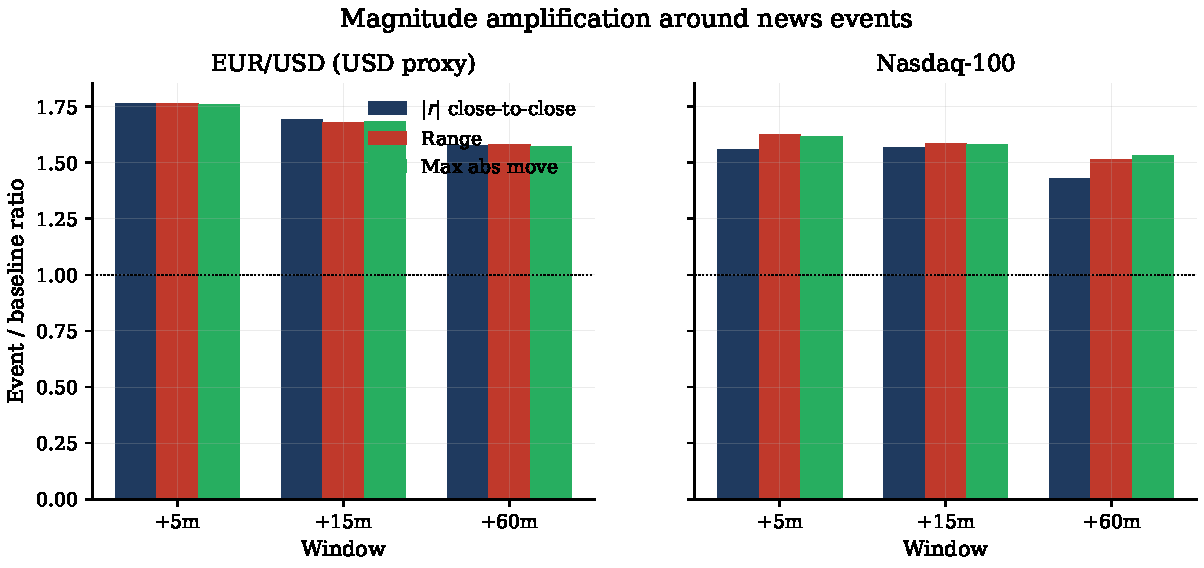
\includegraphics[width=\textwidth]{figures/figure_4_range_ratios.pdf}
\caption{Magnitude amplification: event-window mean divided by
matched-baseline mean for three outcomes at the primary windows.
The horizontal dotted line marks the no-effect level of $1.0$.}
\label{fig:range-ratios}
\end{figure}

\paragraph{C3 (standardised abnormal $z$-scores).}
Re-expressing the same outcomes as standardised abnormal scores
against the hour-of-day, day-of-week matched baseline confirms the
pattern on a dimensionless scale. The mean $|z|$ on the
close-to-close return is in the range $0.57$--$1.24$ across assets
and windows; the mean $|z|$ on range is in the range
$1.04$--$1.53$; and the mean $|z|$ on the maximum absolute move is
in the range $0.92$--$2.40$. The signed return $z$-scores are not
significantly different from zero in most cells, reinforcing the
finding that the news effect is on magnitude rather than on
direction.

\subsection{Direction: modest, and below transaction costs}
\label{ssec:results-direction}

\paragraph{H2 (LLM sentiment hit rate).}
The LLM-derived sentiment label is a weak directional predictor.
Hit rates against the realised target direction range from $49.0$ to
$54.0$ percent across the ten asset-window cells; the largest hit
rate (EUR/USD, 60 minutes, $54.03\%$ on $n = 944$ clusters) is the
only cell that reaches $q < 0.02$. After BH-FDR adjustment, no
other cell survives at $q < 0.05$. The headline picture is
consistent across primary windows: direction is detectable but
small.

\paragraph{C1 (cluster-level direction).}
Aggregating sentiment to cluster level (using the modal sentiment
within each 15-minute cluster) gives the same qualitative pattern
with slightly improved hit rates on the short NDX windows
($53.9\%$ at 5 minutes with $q = 0.012$; $53.2\%$ at 15 minutes
with $q = 0.038$). EUR/USD cluster-level hit rates remain within
sampling noise of $50\%$ at the short windows and improve only at
60 minutes.

\paragraph{LLM versus dictionary and neural baselines.}
A side-by-side comparison of hit rates between the LLM-derived
sentiment, the deterministic Loughran-McDonald dictionary
\citep{loughran2011liability}, and the FinBERT-tone neural
classifier \citep{yang2020finbert}, all computed on identical event
windows, shows that the LLM outperforms both baselines on the
majority of the primary windows. Against Loughran-McDonald, the LLM
advantage is $+0.6$ to $+5.5$ percentage points across the six
primary $5/15/60$-minute cells. Against FinBERT, the LLM advantage
is $-0.5$ to $+4.5$ percentage points; the LLM beats FinBERT in
five of six primary cells and is essentially tied in the sixth
(NDX 15-minute, $-0.5$ pp). On the NDX short windows the dictionary
in fact underperforms a coin flip ($47.0\%$ to $47.8\%$), reflecting
its tendency to map politically-tinged headlines to a uniformly
negative tone that does not correspond to equity-index direction in
the modern period. FinBERT classifies $73.1\%$ of events as neutral
(versus $42.2\%$ for the LLM), reducing its effective directional
sample size by roughly $55\%$ and contributing little incremental
signal where it does commit to a direction.

The LLM also produces cross-asset disagreement
(\texttt{sentiment\_usd} $\neq$ \texttt{sentiment\_ndx}) on $73.5\%$
of events, a property that captures the risk-on/risk-off asymmetry
of macro-news events and that neither the dictionary nor the
single-output FinBERT classifier can express by construction. We
treat this combination of higher hit rates and asset-specific
direction as the principal justification for the LLM methodology
over the standard baselines. Table~\ref{tab:baseline-compare}
reports the three-way comparison cell by cell with Wilson 95\%
confidence intervals, and Figure~\ref{fig:hit-rate-compare} plots
the same information graphically; the LLM bars are above the
$50\%$ reference line in five of the six primary cells, while LM
in particular falls visibly below the reference line on the NDX
short windows.

\begin{table}[!htbp]
\centering
\caption{Direction hit rate: LLM versus baselines.}
\label{tab:baseline-compare}
\begin{threeparttable}
\small
\begin{tabular}{llcccc}
\toprule
\textbf{Asset} & \textbf{Source} & \textbf{Window} & \textbf{$N$} & \textbf{Hit rate} & \textbf{$q$-value} \\
\midrule
EUR/USD & LLM & +5m & 998 & 52.4\%$^{*}$ & 0.342 \\
 & LM (dict.) & +5m & 764 & 51.8\% & 0.618 \\
 & FinBERT & +5m & 437 & 51.9\% & 0.666 \\
\addlinespace[2pt]
 & LLM & +15m & 991 & 52.5\%$^{*}$ & 0.342 \\
 & LM (dict.) & +15m & 758 & 50.4\% & 0.917 \\
 & FinBERT & +15m & 434 & 48.8\% & 0.936 \\
\addlinespace[2pt]
 & LLM & +60m & 944 & 54.0\%$^{***}$ & 0.219 \\
 & LM (dict.) & +60m & 728 & 49.6\% & 0.936 \\
 & FinBERT & +60m & 417 & 51.3\% & 0.780 \\
\addlinespace[2pt]
\midrule
NDX & LLM & +5m & 1,001 & 52.7\%$^{**}$ & 0.342 \\
 & LM (dict.) & +5m & 726 & 47.2\% & 0.986 \\
 & FinBERT & +5m & 417 & 48.2\% & 0.979 \\
\addlinespace[2pt]
 & LLM & +15m & 985 & 51.4\% & 0.666 \\
 & LM (dict.) & +15m & 711 & 47.8\% & 0.986 \\
 & FinBERT & +15m & 409 & 51.8\% & 0.667 \\
\addlinespace[2pt]
 & LLM & +60m & 918 & 49.6\% & 0.936 \\
 & LM (dict.) & +60m & 668 & 47.0\% & 0.986 \\
 & FinBERT & +60m & 388 & 46.6\% & 0.986 \\
\addlinespace[2pt]
\midrule
\bottomrule
\end{tabular}
\begin{tablenotes}
\footnotesize
\item \textit{Notes.} Direction hit rate against the realised target
direction (positive vs negative target return). $N$ counts directional
events (excludes events the classifier labels neutral). Each row
reports a one-sided binomial test against the null $p_0 = 0.5$;
$q$-values from Benjamini-Hochberg FDR adjustment.
$^{*}p<0.10$, $^{**}p<0.05$, $^{***}p<0.01$ on raw $p$-values.
\end{tablenotes}
\end{threeparttable}
\end{table}


\begin{figure}[!htbp]
\centering
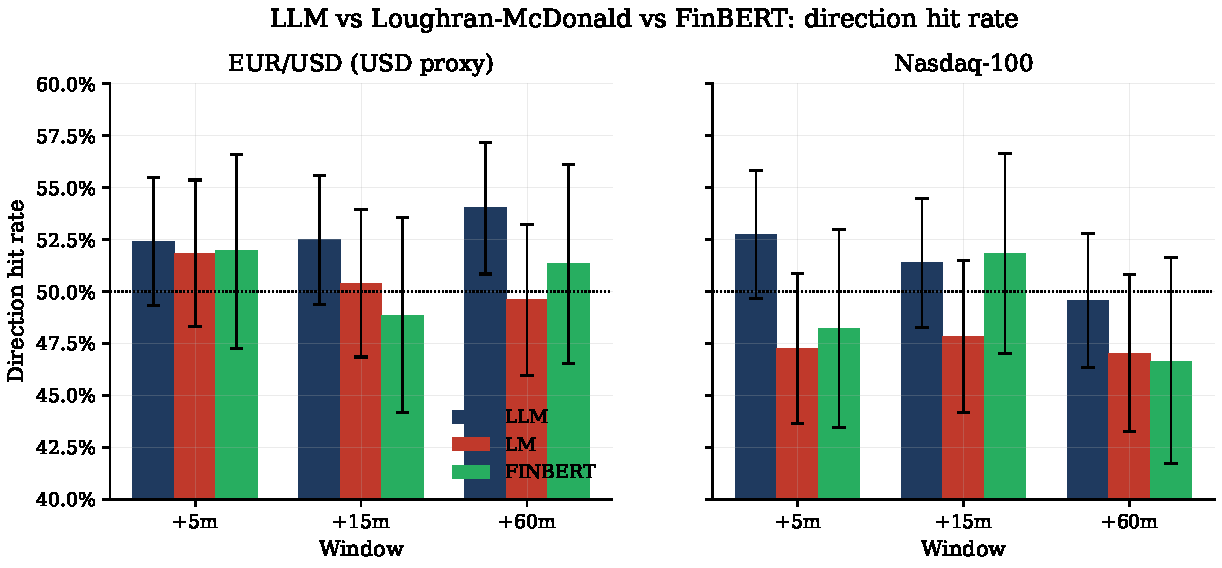
\includegraphics[width=\textwidth]{figures/figure_5_hit_rate_compare.pdf}
\caption{Direction hit rate by classifier, asset, and window, with
Wilson $95\%$ confidence intervals. Horizontal dotted line: the
$50\%$ coin-flip reference. LLM bars are above the reference in
five of six primary cells; the Loughran-McDonald dictionary falls
below the reference on Nasdaq-100 short windows.}
\label{fig:hit-rate-compare}
\end{figure}

\paragraph{Backtest with transaction costs.}
A separate backtest of seven naive sentiment-following strategies,
all with realistic spread and slippage costs, produces negative
cumulative returns and profit factors below $1.0$ on every variant
tested. The same strategies become marginally positive when costs
are removed, which is consistent with the H2/C1 picture: the
directional edge exists but is too small to overcome intraday
execution friction in either asset. We report this as evidence
that the directional signal, while statistically detectable, is not
economically actionable in the form recovered by these labels.
Table~\ref{tab:backtest} reports the full strategy panel and
Figure~\ref{fig:backtest-equity} plots the cumulative equity
curves with and without costs.

\begin{table}[!htbp]
\centering
\caption{Naive sentiment-following strategy backtest with and without transaction costs.}
\label{tab:backtest}
\begin{threeparttable}
\footnotesize
\begin{tabular}{lcrcccc}
\toprule
\textbf{Strategy} & \textbf{Asset} & \textbf{$N$ trades} & \textbf{Win \%} & \textbf{Tot.\,ret.\,(\%)} & \textbf{Profit factor} & \textbf{Max DD (\%)} \\
\midrule
\multicolumn{7}{l}{\textit{With realistic spread + slippage}} \\
no\_chase\_filtered\_hold\_60m & eurusd & 721 & 44.8\% & -5.94 & 0.84 & -6.87 \\
naive\_sentiment\_hold\_60m & eurusd & 1,002 & 46.0\% & -8.58 & 0.85 & -10.03 \\
naive\_sentiment\_hold\_60m & ndx & 960 & 43.6\% & -9.38 & 0.93 & -19.66 \\
naive\_sentiment\_hold\_15m & eurusd & 1,054 & 37.8\% & -11.88 & 0.67 & -12.28 \\
fresh\_sentiment\_breakout\_60m & eurusd & 458 & 35.6\% & -6.71 & 0.35 & -6.76 \\
no\_chase\_filtered\_hold\_15m & eurusd & 767 & 35.6\% & -11.34 & 0.54 & -11.42 \\
fresh\_sentiment\_breakout\_15m & eurusd & 463 & 32.2\% & -6.94 & 0.29 & -6.99 \\
volatility\_breakout\_15m & eurusd & 606 & 34.8\% & -9.63 & 0.30 & -9.64 \\
eurusd\_usd\_1m\_confirmed\_15m & eurusd & 268 & 20.9\% & -4.46 & 0.17 & -4.45 \\
naive\_sentiment\_hold\_15m & ndx & 1,030 & 39.7\% & -19.75 & 0.77 & -22.44 \\
no\_chase\_filtered\_hold\_60m & ndx & 705 & 41.6\% & -16.97 & 0.81 & -21.42 \\
no\_chase\_filtered\_hold\_15m & ndx & 756 & 36.0\% & -20.00 & 0.64 & -22.83 \\
ndx\_cluster\_followthrough\_60m & ndx & 327 & 40.7\% & -8.72 & 0.64 & -10.40 \\
volatility\_breakout\_15m & ndx & 626 & 37.7\% & -21.04 & 0.37 & -21.03 \\
fresh\_sentiment\_breakout\_15m & ndx & 453 & 34.0\% & -17.55 & 0.31 & -17.50 \\
fresh\_sentiment\_breakout\_60m & ndx & 424 & 37.3\% & -16.55 & 0.36 & -16.54 \\
\addlinespace
\multicolumn{7}{l}{\textit{Without transaction costs (frictionless)}} \\
no\_chase\_filtered\_hold\_60m & eurusd & 721 & 52.8\% & 5.60 & 1.18 & -2.89 \\
naive\_sentiment\_hold\_60m & eurusd & 1,002 & 52.6\% & 7.45 & 1.15 & -5.19 \\
naive\_sentiment\_hold\_60m & ndx & 960 & 50.7\% & 29.03 & 1.25 & -10.06 \\
naive\_sentiment\_hold\_15m & eurusd & 1,054 & 50.8\% & 4.98 & 1.19 & -2.81 \\
fresh\_sentiment\_breakout\_60m & eurusd & 458 & 48.3\% & 0.62 & 1.10 & -0.86 \\
no\_chase\_filtered\_hold\_15m & eurusd & 767 & 49.9\% & 0.94 & 1.05 & -3.15 \\
fresh\_sentiment\_breakout\_15m & eurusd & 463 & 48.6\% & 0.47 & 1.09 & -0.80 \\
volatility\_breakout\_15m & eurusd & 606 & 49.3\% & 0.07 & 1.01 & -1.19 \\
eurusd\_usd\_1m\_confirmed\_15m & eurusd & 268 & 44.0\% & -0.17 & 0.94 & -0.54 \\
naive\_sentiment\_hold\_15m & ndx & 1,030 & 53.2\% & 21.46 & 1.33 & -7.38 \\
no\_chase\_filtered\_hold\_60m & ndx & 705 & 50.1\% & 11.23 & 1.15 & -5.98 \\
no\_chase\_filtered\_hold\_15m & ndx & 756 & 51.7\% & 10.24 & 1.27 & -3.93 \\
ndx\_cluster\_followthrough\_60m & ndx & 327 & 44.6\% & 4.36 & 1.26 & -2.30 \\
volatility\_breakout\_15m & ndx & 626 & 55.6\% & 4.00 & 1.20 & -1.35 \\
fresh\_sentiment\_breakout\_15m & ndx & 453 & 50.1\% & 0.58 & 1.04 & -1.27 \\
fresh\_sentiment\_breakout\_60m & ndx & 424 & 50.2\% & 0.41 & 1.02 & -1.47 \\
\bottomrule
\end{tabular}
\begin{tablenotes}
\footnotesize
\item \textit{Notes.} Seven naive sentiment-following strategies
applied to each event, traded with EUR/USD spot or NDX CFD prices.
Costs include venue-typical spread and slippage. Total return is
the simple sum across trades, in percentage points. Profit factor
is gross profit divided by gross loss; values below 1.0 indicate
a losing strategy.
\end{tablenotes}
\end{threeparttable}
\end{table}


\begin{figure}[!htbp]
\centering
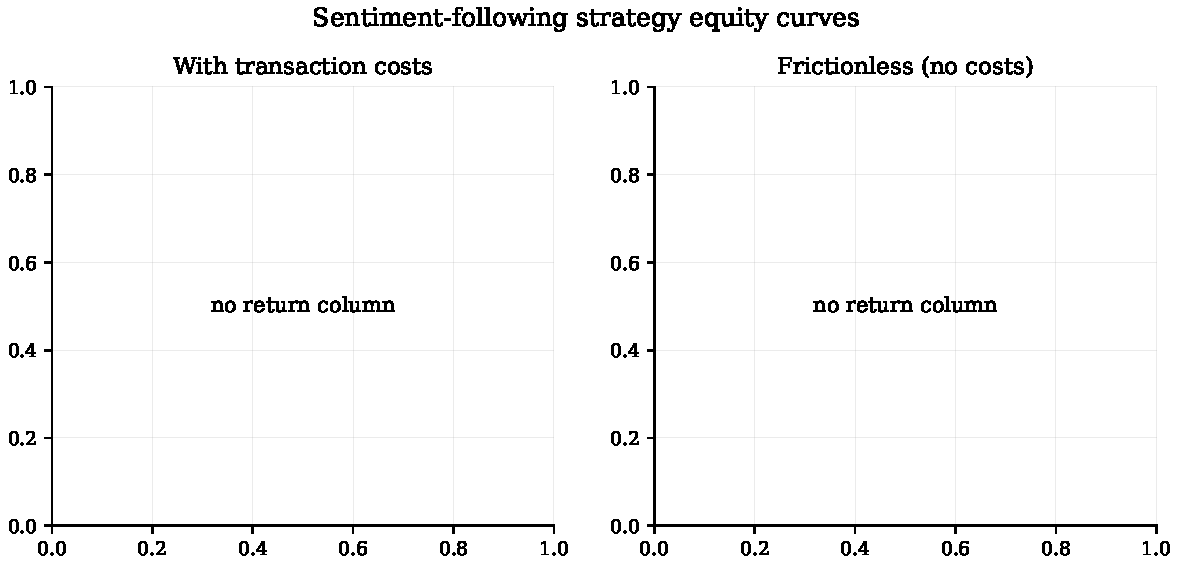
\includegraphics[width=\textwidth]{figures/figure_9_backtest_equity.pdf}
\caption{Cumulative equity curves for seven naive sentiment-following
strategies traded on each asset, with realistic transaction costs
(left) and frictionless (right). All cost-included strategies trend
downward over the sample.}
\label{fig:backtest-equity}
\end{figure}

\subsection{Heterogeneity by category and time of day}
\label{ssec:results-heterogeneity}

\paragraph{C4 (per-category targeted tests).}
Across the five non-trivial categories (\texttt{central\_bank},
\texttt{geopolitical}, \texttt{politics}, \texttt{energy},
\texttt{corporate}), the volatility-magnitude finding of
Section~\ref{ssec:results-volatility} holds uniformly: standardised
abnormal $z$-scores on the maximum absolute move are significantly
positive at $q < 10^{-9}$ in every category-asset-window cell we
tested. The directional content is more mixed: central-bank events
on the NDX 15-minute window achieve a hit rate of $55.8\%$ with
$q = 0.058$, but no other single category-asset-window cell reaches
$q < 0.05$ on direction. The pattern is that category-level
information helps locate where the magnitude reaction is largest
(central-bank releases produce the highest absolute moves on
EUR/USD, geopolitical events the highest on NDX) without sharpening
direction in a transportable way. Figure~\ref{fig:sentiment-heatmap}
visualises the cross-asset sentiment composition by category: USD
and NDX shares differ markedly within \texttt{geopolitical} and
\texttt{politics} (the risk-on/risk-off categories), while
\texttt{central\_bank} events show the most pronounced cross-asset
divergence.

\begin{figure}[!htbp]
\centering
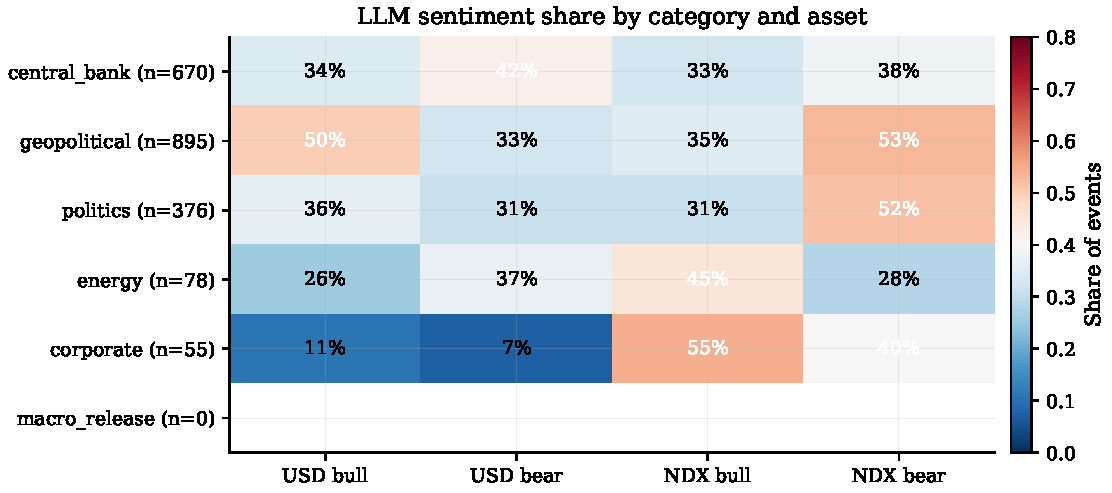
\includegraphics[width=0.78\textwidth]{figures/figure_6_sentiment_heatmap.pdf}
\caption{Share of LLM-labelled bull and bear events within each
category, separately for the USD and NDX targets. Cells are
percentages of the category total. Risk-off categories
(\texttt{geopolitical}, \texttt{central\_bank}) show the largest
cross-asset asymmetry.}
\label{fig:sentiment-heatmap}
\end{figure}

\paragraph{H11 (time-of-day and day-of-week).}
EUR/USD shows a robust hour-of-day effect on the event/baseline
ratio (Kruskal-Wallis $p < 10^{-12}$, $q < 10^{-11}$), with the
largest effects clustered around the New York open. The day-of-week
effect is not statistically significant. NDX shows neither effect
at a level that survives FDR correction; we attribute this to the
more uniform liquidity profile of the index relative to a single
currency pair.

\subsection{Timing and persistence}
\label{ssec:results-timing}

\paragraph{H8 (pre-event drift).}
The absolute return in the 15 minutes preceding an event is
significantly elevated above the matched baseline on both assets:
EUR/USD mean pre-event $|r| = 0.053$ versus baseline $0.031$
($q < 10^{-46}$), NDX $|r| = 0.158$ versus baseline $0.092$
($q < 10^{-40}$). The pre-event drift is on the same order of
magnitude as the post-event drift for the same windows.
Figure~\ref{fig:pre-post-drift} plots the per-minute mean $|r|$
from $-30$ to $+30$ minutes around each event; the lift starts
visibly before the event timestamp on both assets, particularly
in the final five minutes. We interpret this finding cautiously:
the Discord timestamp is the timestamp at which the
FinancialJuice account posts the headline, not the timestamp of
the underlying primary source (wire service, agency feed,
official release). The most plausible reading of the pre-event
drift is information arrival latency in the public feed rather
than insider trading or front-running, but the data alone cannot
adjudicate between these. Practitioners reading this section
should infer that entering a trade at the timestamp of the
Discord post is often already late.

\begin{figure}[!htbp]
\centering
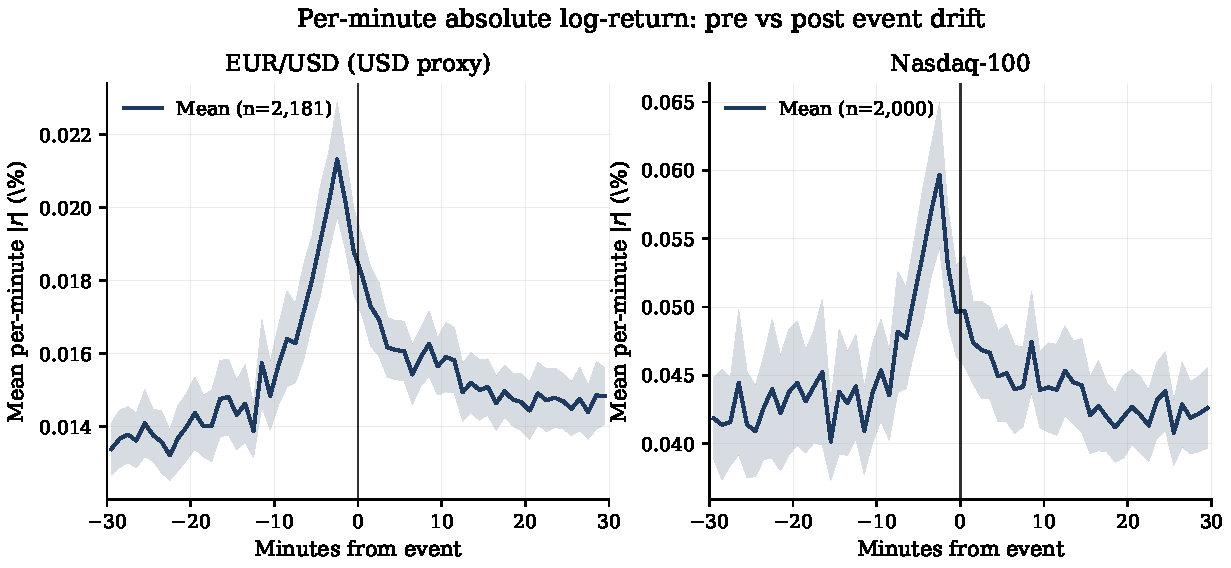
\includegraphics[width=\textwidth]{figures/figure_7_pre_post_drift.pdf}
\caption{Mean per-minute $|r|$ in a $\pm 30$-minute window around
each event. Shaded area: $\pm 1.96$ standard errors of the cross-event
mean. Vertical line: event timestamp. The lift visibly precedes
the timestamp on both assets.}
\label{fig:pre-post-drift}
\end{figure}

\paragraph{H9 (sign persistence between $+15$m and $+4$h).}
Across both assets, the sign of the $+15$-minute return agrees with
the sign of the $+4$-hour return on $57.6\%$ of events
($q < 10^{-4}$ on both assets). The median absolute size ratio
between the two windows is $3.1\times$ for EUR/USD and $4.5\times$
for NDX, indicating that the initial move is typically extended
(not reversed) over the subsequent several hours.
Figure~\ref{fig:sign-persistence} plots the $+15$-minute target
return against the $+4$-hour return; the bulk of points sits in
the first and third quadrants (sign agreement), and the slope is
visibly positive.

\begin{figure}[!htbp]
\centering
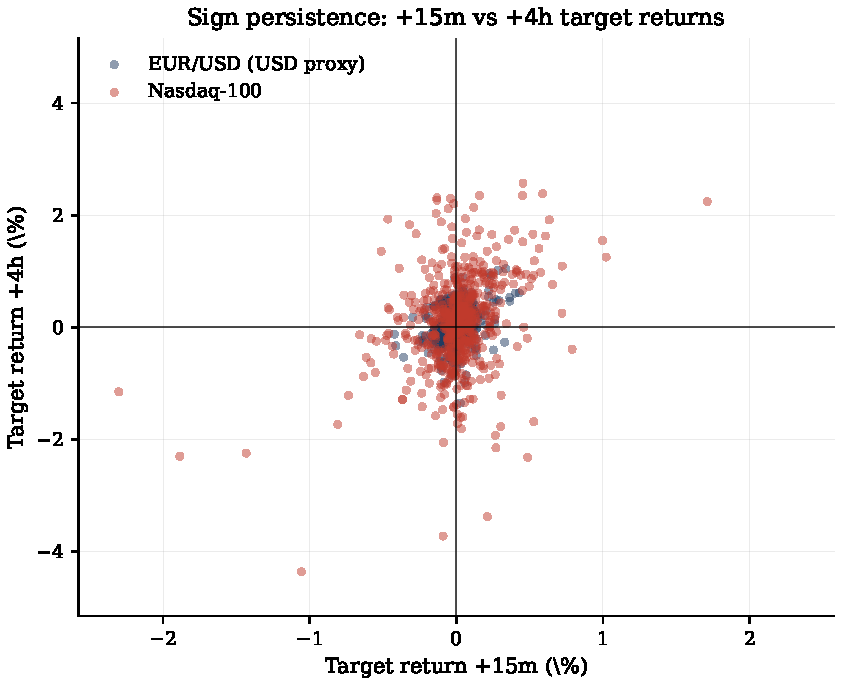
\includegraphics[width=0.7\textwidth]{figures/figure_8_sign_persistence.pdf}
\caption{Target return at $+15$ minutes versus at $+4$ hours. Each
point is one event-asset pair; colour distinguishes the two
assets. Quadrants I and III correspond to sign agreement; the
sample concentrates there at $57.6\%$ of events.}
\label{fig:sign-persistence}
\end{figure}

This is a useful complement to
Section~\ref{ssec:results-direction}: while direction is hard to
predict, conditional on a move having occurred in the first
quarter-hour, it is more likely to be extended than reversed over
the rest of the trading session.

\subsection{Market structure}
\label{ssec:results-market-structure}

\paragraph{H4 (closed-period gap).}
When markets are closed (weekends, holidays), we aggregate the
target sentiment of events occurring within the closed period and
regress the realised opening gap on the aggregate sentiment. On
NDX, the coefficient is $+0.268$ with $q = 0.021$ on 92 closed
periods ($R^2 = 7.7\%$); on EUR/USD the coefficient is $+0.102$
with $q = 0.054$ on 32 periods ($R^2 = 10.3\%$). The NDX result is
the cleaner of the two, consistent with the longer official
non-trading window for equities than for FX.

\paragraph{H14 (cross-asset).}
The Pearson correlation between EUR/USD event-window returns and
NDX event-window returns at 15 minutes is $-0.148$ ($q < 10^{-6}$),
as expected from the macroeconomic risk-on/risk-off pattern under
which USD strength tends to coincide with NDX weakness.
Re-expressed in the USD-proxy convention, the correlation becomes
$+0.148$ and the sign-match rate (USD-proxy and NDX moving in the
same direction) is $56.6\%$ across $1{,}176$ clusters
($q < 10^{-5}$). We report both signs to forestall
misinterpretation when the paper is read alongside event studies
that work directly with the EUR/USD price.

\subsection{Robustness}
\label{ssec:results-robustness}

The Sections~\ref{ssec:results-volatility}--\ref{ssec:results-market-structure}
results are supported by three robustness exercises.

\paragraph{C5 (pre/post 2026-01-15 knowledge-cutoff split).}
Splitting the sample at the LLM's training data cutoff, the central
magnitude findings hold on both halves with $q < 10^{-13}$
throughout. On the pre-cutoff half, mean $|z|$ for the absolute
return is $0.80$--$1.00$ across primary windows on EUR/USD and
$0.64$--$0.83$ on NDX; the post-cutoff half is statistically
similar. This argues against an explanation in which the LLM's
effect is driven by memorisation of training-period news. Direction
hit rates on the post-cutoff half remain within the same modest
range reported in Section~\ref{ssec:results-direction}; the NDX
5-minute pre-cutoff hit rate is $55.8\%$ with $q = 0.002$.

\paragraph{C6 (multivariate controls).}
A multivariate OLS of the standardised abnormal $|z|$ on category
dummies, surprise level, expected magnitude, LLM confidence,
$\log(\text{cluster size})$, mean headline length, and pre-event
move, with cluster-robust standard errors, recovers two controls
that are consistently informative across cells:
$\log(\text{cluster size})$ ($q < 0.02$ in the EUR/USD 5-minute
cell) and pre-event drift ($q < 0.002$ in the same cell). The
cluster-size finding implies that larger news bursts produce larger
reactions on average, even controlling for the sentiment and
category labels. The pre-event-drift control complements the H8
result by showing that the event-window reaction is partially
predictable from the run-up to the event. Category dummies absorb
the energy and corporate effects identified in C4.
Table~\ref{tab:multivariate} reports four representative cells.

\begin{table}[!htbp]
\centering
\caption{Multivariate regression of standardised abnormal magnitude.}
\label{tab:multivariate}
\begin{threeparttable}
\small
\begin{tabular}{lcccc}
\toprule
 & \multicolumn{2}{c}{EUR/USD ($|z|$)} & \multicolumn{2}{c}{NDX ($|z|$)} \\
\cmidrule(lr){2-3} \cmidrule(lr){4-5}
Term & +5m & +60m & +5m & +60m \\
\midrule
$\log(\text{cluster size})$ & $1.925$$^{**}$ & $1.522$$^{***}$ & $1.057$$^{***}$ & $0.593$$^{*}$ \\
 & $(0.751)$ & $(0.413)$ & $(0.367)$ & $(0.323)$ \\
\addlinespace[2pt]
Pre-event $|r|_{15}$ & $8.516$$^{***}$ & $3.954$$^{***}$ & $3.529$$^{***}$ & $2.386$$^{**}$ \\
 & $(2.480)$ & $(1.337)$ & $(0.954)$ & $(0.956)$ \\
\addlinespace[2pt]
Surprise level & $-0.010$ & $-0.239$ & $0.139$ & $-0.228$ \\
 & $(0.259)$ & $(0.194)$ & $(0.140)$ & $(0.167)$ \\
\addlinespace[2pt]
Expected magnitude & $0.366$ & $0.377$$^{*}$ & $-0.081$ & $0.257$ \\
 & $(0.241)$ & $(0.206)$ & $(0.153)$ & $(0.199)$ \\
\addlinespace[2pt]
LLM confidence & $-0.031$ & $-0.004$ & $0.001$ & $0.814$ \\
 & $(0.862)$ & $(0.829)$ & $(0.687)$ & $(1.028)$ \\
\addlinespace[2pt]
Headline length & $-0.001$ & $0.001$ & $-0.001$$^{*}$ & $-0.001$$^{*}$ \\
 & $(0.001)$ & $(0.001)$ & $(0.000)$ & $(0.000)$ \\
\addlinespace[2pt]
Cat: central bank & -- & -- & -- & -- \\
 &  &  &  &  \\
\addlinespace[2pt]
Cat: geopolitical & $-0.744$$^{**}$ & $-0.393$$^{*}$ & $-0.104$ & $-0.157$ \\
 & $(0.299)$ & $(0.213)$ & $(0.169)$ & $(0.199)$ \\
\addlinespace[2pt]
Cat: corporate & $-0.876$$^{*}$ & $-0.631$$^{*}$ & $-0.262$ & $0.029$ \\
 & $(0.447)$ & $(0.332)$ & $(0.249)$ & $(0.345)$ \\
\addlinespace[2pt]
Cat: energy & $-0.952$$^{***}$ & $-0.124$ & $-0.189$ & $-0.399$ \\
 & $(0.290)$ & $(0.316)$ & $(0.190)$ & $(0.248)$ \\
\addlinespace[2pt]
\midrule
$R^2$ & 0.122 & 0.097 & 0.193 & 0.096 \\
$N$ clusters & 1,279 & 1,202 & 1,188 & 1,088 \\
\bottomrule
\end{tabular}
\begin{tablenotes}
\footnotesize
\item \textit{Notes.} OLS of the standardised abnormal $|z|$ on the
listed regressors. Coefficient on top, robust standard error in
parentheses below; cluster-robust covariance with the 15-minute
news-cluster identifier as the grouping variable.
$^{*}p<0.10$, $^{**}p<0.05$, $^{***}p<0.01$ on raw $p$-values;
$q$-values reported in the Online Appendix. Category baseline:
\texttt{politics}.
\end{tablenotes}
\end{threeparttable}
\end{table}


\begin{table}[!htbp]
\centering
\caption{Stability across LLM knowledge-cutoff split (15 January 2026).}
\label{tab:pre-post}
\begin{threeparttable}
\small
\begin{tabular}{lcccccc}
\toprule
 & \multicolumn{3}{c}{EUR/USD} & \multicolumn{3}{c}{NDX} \\
\cmidrule(lr){2-4} \cmidrule(lr){5-7}
Period & 5m & 15m & 60m & 5m & 15m & 60m \\
\midrule
Pre-cutoff: mean $|z|_{\,|r|}$ & 0.982 & 0.895 & 0.899 & 0.644 & 0.680 & 0.638 \\
Post-cutoff: mean $|z|_{\,|r|}$ & 0.736 & 0.726 & 0.521 & 0.495 & 0.535 & 0.411 \\
Pre-cutoff: $q$ & $1.9\!\times\!10^{-15}$ & ${<}10^{-15}$ & ${<}10^{-15}$ & $1.7\!\times\!10^{-15}$ & $7.8\!\times\!10^{-15}$ & $2.4\!\times\!10^{-13}$ \\
Post-cutoff: $q$ & $1.7\!\times\!10^{-10}$ & $3.9\!\times\!10^{-11}$ & $2.3\!\times\!10^{-8}$ & $1.2\!\times\!10^{-8}$ & $3.1\!\times\!10^{-11}$ & $5.7\!\times\!10^{-7}$ \\
\addlinespace
Pre-cutoff $N$ clusters & 901 & 891 & 849 & 839 & 827 & 774 \\
\bottomrule
\end{tabular}
\begin{tablenotes}
\footnotesize
\item \textit{Notes.} Standardised abnormal absolute return $|z|$
in the pre-cutoff and post-cutoff halves, with the split at the LLM's
reported training data cutoff of 15 January 2026. $q$-values from
one-sided $t$-test against zero with BH-FDR adjustment.
\end{tablenotes}
\end{threeparttable}
\end{table}


\paragraph{C7 (winsorisation at the 1\% tails).}
Winsorising every outcome at the $1\%$ tails produces mean $|z|$
values that are within $5$--$10\%$ of the raw mean and $p$-values
that remain below $10^{-30}$ in the central cells. The headline
magnitude finding is not driven by a small number of extreme
observations. Table~\ref{tab:winsor} reports the raw and
winsorised means side by side.

\begin{table}[!htbp]
\centering
\caption{Robustness to winsorisation at 1\% tails.}
\label{tab:winsor}
\begin{threeparttable}
\small
\begin{tabular}{lccccccc}
\toprule
 & & \multicolumn{2}{c}{Mean $|z|$} & \multicolumn{2}{c}{$q$-value ($t$-test)} \\
\cmidrule(lr){3-4} \cmidrule(lr){5-6}
Asset & Window & Raw & Winsor 1\% & Raw & Winsor 1\% & $N$ \\
\midrule
EUR/USD & +5m & 0.908 & 0.790 & ${<}10^{-15}$ & ${<}10^{-15}$ & 1,286 \\
EUR/USD & +15m & 0.844 & 0.757 & ${<}10^{-15}$ & ${<}10^{-15}$ & 1,271 \\
EUR/USD & +60m & 0.787 & 0.709 & ${<}10^{-15}$ & ${<}10^{-15}$ & 1,207 \\
NDX & +5m & 0.599 & 0.549 & ${<}10^{-15}$ & ${<}10^{-15}$ & 1,198 \\
NDX & +15m & 0.637 & 0.589 & ${<}10^{-15}$ & ${<}10^{-15}$ & 1,176 \\
NDX & +60m & 0.571 & 0.527 & ${<}10^{-15}$ & ${<}10^{-15}$ & 1,097 \\
\bottomrule
\end{tabular}
\begin{tablenotes}
\footnotesize
\item \textit{Notes.} Mean of $|z|$ (standardised abnormal absolute
return) in the raw and 1\%-winsorised samples, with corresponding
$q$-values from a one-sided $t$-test against zero. Winsorisation
is applied separately within each (asset, window) cell.
\end{tablenotes}
\end{threeparttable}
\end{table}


\paragraph{Auxiliary LLM labels.}
The LLM's \texttt{expected\_magnitude} and \texttt{surprise\_level}
labels (consolidating H5 and H13) have modest additional
explanatory power, with ANOVA $F$-statistics that are significant
at $q < 0.05$ on a minority of cells, primarily for NDX short
windows. We report the full table in the Online Appendix but
recommend treating these labels as exploratory rather than as core
inputs.
